\documentclass[a4paper,12pt]{article}
\usepackage[utf8]{inputenc}
\usepackage[T1]{fontenc}
\usepackage[english]{babel}
\usepackage{indentfirst}
\usepackage{graphicx}
\usepackage{amsmath}
\usepackage{amsthm}
\usepackage{amssymb}
\usepackage{fancyhdr}
\newtheorem{tetel}{Theorem}
\newtheorem{defi}{Definition}
\frenchspacing
\begin{document}
\pagestyle{fancy}
\begin{center}

\includegraphics[width=1.8cm]{elte.jpg}

\includegraphics[width=1.8cm]{eit.jpg}
\end{center}
\lfoot{}
\rfoot{}
\chead{A lightweight Bitcoin client}
\rhead{}
\lhead{}
\begin{center}
\LARGE{\textbf{Distributed Robust Accounting}}\\
\vspace{0.5cm}
\textbf{\large{Applied Cryptography Project}}\\
\vspace{0.5cm}
\end{center}
\begin{tabular}{p{2cm}l}
\underline{Authors}:&Réka Szabó \textit{(szreka327@gmail.com)}\\
&Balázs Pejó \textit{(balazs.pejo@gmail.com)}\\
&Máté Horváth \textit{(er.mate@gmail.com)}
\end{tabular}
\section{Motivation}
Bitcoin is an experimental, decentralized digital currency that enables instant payments to anyone, anywhere in the world. Bitcoin uses peer-to-peer technology to operate with no central authority: managing transactions and issuing money are carried out collectively by the network. Bitcoin is designed around the idea of using cryptography to control the creation and transfer of money, rather than relying on central authorities.

\begin{figure}[h]\label{size}
\begin{center}
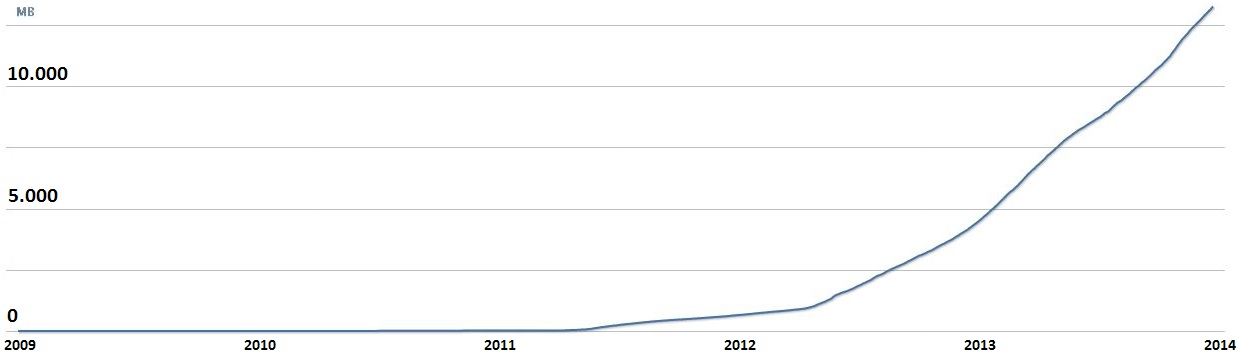
\includegraphics[width=10cm]{blockchainsize.jpg}
\caption{The size of the data that needs syncronization.}
\end{center}
\end{figure}
\vspace{-0.5cm}

However, Bitcoin requires that every node stores the entire ledger and broadcasts every transaction to every node. This limits the scalability of the system and also constitutes an entry barrier: it takes many hours for a new installation to download the entire block chain (which is how the transaction ledger is called in Bitcoin terminology) as Figure \ref{size}. shows. Except for the most expensive models, cellphones do not have the storage capacity to store all the transactions and it is also often prohibitively expensive in terms of mobile communication to maintain a bitcoin network node on a cellphone. At present, this implies that mobile devices and other low-power computers must trust one or more nodes on the bitcoin network which is slowly but surely turning into a centralized structure quite out of line with its original ethos.

On the other hand, Bitcoin's design includes several features that seem to be aimed at decentralization, allowing nodes to hold only partial copies of the block chain and still not trust other nodes for verifying its integrity regarding transactions and accounts of interest. The goal of this project is to design and maybe prototype such decentralization.

\section{Background}

In this section we summarize the how a regular full node works. The basic problem Bitcoin solves is achieving consensus on who owns what. Nodes maintains a database of unspent outputs, and transactions that attempt to spend outputs that do not exist or were already spent are ignored. Blocks are solved by miners and broadcast to ensure everyone agrees on the ordering of transactions, and so nodes that do not see a broadcast transaction for some reason (eg, they were offline at the time) can catch up.

The act of checking, storing and updating the database for every single transaction is quite intensive. Catching up to the current state of the database from scratch is also very slow. For this reason, not every computer can run a full node.

Transactions in each block of the block chain are hashed in a so-called Merkle tree (Figure \ref{merkle}), which can be used to verify any transaction without having to download all. 

\begin{figure}[h]\label{merkle}
\begin{center}
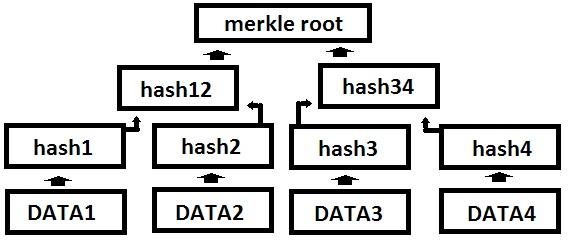
\includegraphics[width=8cm]{mroot.jpg}
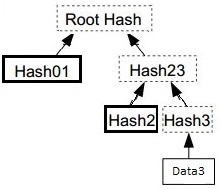
\includegraphics[width=4cm]{branch.jpg}
\caption{The structure of a Merkle tree, and the Merkle branch of a data.}
\end{center}
\end{figure}
\vspace{-0.5cm}

Every transaction has a hash associated with it. In a block, all of the transaction hashes in the block are themselves hashed (sometimes several times - the exact process is complex, details can be found in [\ref{shatoshi}]), and the result is the Merkle root. In other words, the Merkle root is the hash of all the hashes of all the transactions in the block. 

The Merkle root is included in the block header. With this scheme, it is possible to securely verify that a transaction has been accepted by the network (and get the number of confirmations) by downloading just the tiny block headers and Merkle tree - downloading the entire block chain is unnecessary. This feature is currently not used in Bitcoin. 

Each node is particularly and primarily interested in transactions that concern the accounts that are controlled by their operators, perhaps some watched accounts (such as those of counterparties). It needs to verify that all the transactions preceding them beginning with emission (mining) have been arithmetically correct and that no double spending has been attempted. It may also verify random transactions as a means of
spot-checking the network.

\section{Solution}
The solution is a simplified Bitcoin client that does not store all the transaction and the blockchain, only transactions that are relevant to the wallet are stored. Every other transaction is thrown away or simply never downloaded. The block chain is still used and broadcast transactions are still received, but those transactions are not and cannot be checked to ensure they are valid. This mode of operation is fast and lightweight enough to be run on a smartphone.

\subsection{Basics}
Each balance is simply associated with an address and its public-private key pair. The money "belongs" to anyone who has the private key and can sign transactions with it. Moreover, those keys do not have to be registered anywhere in advance, as they are only used when required for a transaction. Each person can have many such addresses, each with its own balance, which makes it very difficult to know which person owns what amount. The Bitcoin software encourages this behavior by default.

When someone starts to use this simplified wallet, it generates new public-private key pairs, so it knows the creation time of all its keys. To keep track of its future transactions, block contents before this time do not have to be downloaded, only the headers, so it is much faster to bootstrap the system in this way. The method is similar to bitcoinj's fast catchup. This way it is possible to synchronize with the chain just by downloading headers and some transactions and Merkle branches, but sometimes this is still too slow. 

It can further be augmented with bitcoinj's chekpoint files. These are generated using the BuildCheckpoints tool that can be found in the tools module of the bitcoinj source code. BuildCheckpoints downloads headers and writes out a subset of them to a file. That file can then be shipped with your application. When you create a new BlockStore object, you can use that file to initialize it to whichever checkpointed block comes just before your wallets fast catchup time (i.e. the birthday of the oldest key in your wallet). Then you only need to download headers from that point onwards.

% Checkpoints are called checkpoints because, like the upstream Satoshi client, once you've initialized the block store with one bitcoinj will refuse to re-organise (process chain splits) past that point. In fact, it won't even recognize that a re-org has taken place because the earlier blocks don't exist in the block store, thus the alternative fork of the chain will be seen merely as a set of orphan blocks. For this reason the BuildCheckpoints tool won't add any checkpoints fresher than one month from when it's run - it only takes a few seconds to download the last months worth of chain headers, and no fork is likely to ever be longer than one month.

When a transaction is broadcast over the network we say it is pending inclusion in a block. Mining nodes will check it for themselves and if it is valid, include it in the current block they are trying to solve. Nodes do not relay invalid transactions. The lightweight bitcoin client will receive pending transactions, add them to the wallet, and run event listeners. 

% Mivel mi DHT-t használunk, ezért Bloom filtert használni arra, hogy a sajátjaidon kívül más tranzakciót is eltárolj nem lehetséges, mivel a DHT elég jól meghatározza, hogy pontosan milyen ranzakciókat tárolj el. Egy ilyen Bloom filter esetén a többi node nem tudná hogy kinél keressen egy adott tranzakciót, mindenkit végig kéne kérdezni. arra viszont, hogy a saját tranzakcióinkat eltároljuk hasznos lehet, mert gondolom gyorsabb ezzel ellenőrizni mondjuk egy blokk kihirdetésénél hogy benne van-e a mienk. viszont adhat false pozitívta, de ez sem baj, mert akkor eltárolunk még pluszba néhány random tranzakciót, ez nem fogja befolyásolni a rendszer működését.

\subsection{Data storage}
Nodes operating this way can form a system that stores each transaction of the network and does not rely on other nodes to verify the integrity of transactions they are interested in.

Each node stores transactions that concern the accounts that are controlled by their operators. Furthermore, they store some other transaction, so an eavesdropper will not be able to decide which transaction (public key) belongs to the node. If there is a sufficiently large number (as defined in Chapter \ref{number}) of simplified nodes in the network, they will be able to store every bitcoin transaction. If a node needs some information on a specific transaction, it will send a request to the node that stores this transaction, and that node will reply with the requested information.

The main question is how to distribute the transactions among the nodes in a way they can easily find which node stores which transactions.
The solution is based on distributed hash tables. 

A distributed hash table (DHT) is a class of a decentralized distributed system that provides a lookup service similar to a hash table; (key, value) pairs are stored in a DHT, and any participating node can efficiently retrieve the value associated with a given key. Responsibility for maintaining the mapping from keys to values is distributed among the nodes, in such a way that a change in the set of participants causes a minimal amount of disruption. This allows a DHT to scale to extremely large numbers of nodes and to handle continual node arrivals, departures, and failures. DHT forms an infrastructure that can be used to form peer-to-peer content distribution [\ref{dhtwiki}].

\newpage

In this network the hash of a transaction will play the role of the key, and the raw transaction will be the value. When there is a new transaction, each node forwards it through the network until it reaches the node responsible for it. That node then stores the transaction. Another node can retrieve this transaction by sending a request message with the hash of the transaction. This message is forwarded by the other nodes, until it reaches the node that stores the transaction. This node will reply with the raw transaction.

% itt azt nem tudom, hogy ha egy node-nek kell egy raw tranzakció, akkor azt mi alapján tudja lekérni. pl lehet h a hashét pont nem tudja, csak más adatokat róla... na most itt lehetséges-e nem hash alapján keresni? hát sztem nem nagyon... bár egy node-ot nyilván az ő tranzakciói érdeklik, amiről tud minden adatot, csak azt nem hogy benne van-emár egy blokkban. ez esetben csak emiatt akar körbeérdeklődni a tranzakcióról, és ekkor tudja ezt a hash-el csinálni. de más esetekben nem tudom hogy kéne 

We need to define how to partition the keyspace and find a proper routing protocol.

\subsection{Key space partitioning}

We need to map the hash of transactions to some node id.

Nodes identify themselves and find other nodes by the IMEI (International Mobile Equipment Identity) number of the device. Following the original Bitcoin protocol, which stores the IP addresses of nodes they previously connected to in their local peers.dat file, the IMEI numbers can be stored in a similar way. So the simplest way is to use IMEI numbers as node ids in the keyspace partitioning.

A transaction hash is a 32 bytes hexadecimal number, we need to map them to IMEI numbers. An easy way is to calculate the SHA256 hash of the IMEI numbers, and the node with the closest hash value to the transaction hash will store the transaction.

We treat the keys (hash of IMEI numbers) as points on a circle and define the distance of two keys as the distance traveling clockwise on the circle from one key to the other. So the circular keyspace is cut into contiguous segments whose end points are the hash of node ids (IMEI numbers). If $id_1$ and $id_2$ are two adjacent node ids, with a shorter clockwise distance from $id_1$ to $id_2$ then $id_1$ will store all the values between $id_1$ and $id_2$. (Like in the chord DHT.)

Since values of a hash function are uniformly distributed, node ids will be uniformly distributed in the keyspace. It implies that nodes will have to store the about same amount of transactions.

% itt a következő a problémám: ha valaki megfigyeli egy node forgalmát (h milyen tranzakciókat tárol el) akkor mivel nem csak a sajátját tárolja el nem tudja h mik az ő tranzakciói. de a tarnzakciók azonosítójából ki tudja szűrni h azt a node azért tárolta-e el mert közel van az id-jéhez vagy mert az övé a tranzakció. erre ugye megoldás lenne h a node nem hozza nyilvánosságra az id-jét, de ekkor a későbbiekben leírt routingot nem lehetne megvalósítani... vagy persze egymás között eltitkosítva küldözgetnek üzenetet, gondolom ez amúgy is így van, de... hát szóval ez megint csak problémákat vet fel

\subsection{Routing protocol}

A suitable routing protocol is necessary for forwarding and requesting transactions and adding and deleting nodes.

A node can send messages to nodes whose IMEI number is known to it (stored in its local peers.dat). For these nodes it can calculate their id (hash of IMEI number).

If a new node is added to the network,  it first finds some nodes already in the system. The new node sends its id  (in this chapter we refer as id to to the hash of IMEI numbers) to these nodes. These nodes will find in their peer.dat database the node which id is closest to this node's id in the sense of the above defined distance (they hash the stored IMEI numbers and check it), and forward the message to it. If this node can find another node closer to this new node it will forward this message, and so on until the message reaches the node closest to the new node. This node will not find anyone closer to the new node, so it will not forward the message.

This node decrease its key space (so part of the transactions that were previously stored by this node will be stored by the new node) and sends a message to the new node with its id, part of its transactions and the range of transaction hashes it should store later; furthermore it stores this new node as its children. The new node will store this node as its father

Example: $id_1$ and $id_2$ are two adjacent nodes, and $id_3$ is a newly arrived node such that $id_3$ is between $id_1$ and $id_2$. In this case a message will reach $id_1$ with the new nodes id. $id_1$ know checks that its closer to it than to $id_2$. It sends its own is ($id_1$) to $id_3$ along with $id_2$ and the transactions between $id_3$ and $id_2$ (they were stored by $id_1$ but from now on they will be stored by $id_3$). From $id_2$ $id_3$ will know that the transactions it should store range from $id_3$ to $id_2$.

This way the new node will know which transactions it should store in the future and will store some other transaction in its database. Furthermore it knows its two neighbours, so if a routing message arrives to it the node will be able to decide which way to forward it.

This new node will also store the id of the nodes it sent the first message to. This way the node will know nodes further to it, not only its neighbors. This will fasten up a routing and in the future if it gets a message from a new node, it will store its id as well.

If a node leaves the system, it notifies its father node and its children. It sends the children the id of its father node, and the children will store it as their new father. It sends a message to the father with all its stored transactions and the children ids. The father will redistribute the transactions among its children. 

A routing protocol: assume that node A wants to find a transaction. It sends a request message with the transaction hash to the node in its peer.dat file whose id is closest to the transaction hash. This node will forward this transaction hash with the id of the original node to the node in its peer.dat file with the closest id to the hash and so on, until it reaches the node who actually stores that transaction. This node will send a the transaction to the original node and stores this node's id.

Basically, if a node gets a message from a node previously unknown to it it will store its id.

When broadcasting a transaction a node stores the ones that belong to him or that are close to him. When broadcasting a block each node stores the block header and checks the transactions in it and stores Merkle branches of the previously stored transactions. Since nodes stores all the block headers, with the Merkle branch they can verify a transaction.

The transactions controlled by the owner of the wallet are stored via Bloom filters. A Bloom filter is a compact, privacy preserving representation of the keys/addresses in a wallet. When one is passed to a remote peer, it changes its behavior. Instead of relaying all broadcast transactions and the full contents of blocks, it matches each transaction it sees against the filter. If the filter matches, that transaction is sent to your app, otherwise it is ignored. When a transaction is being sent to you because it is in a block, it comes with a Merkle branch that mathematically proves the transaction was included in that block. BitcoinJ checks the Merkle branch for each transaction, and rejects any attempts to defraud you.

\subsection{First steps}
The DHT method works only if there is a sufficiently large network of these simplified clients. Until that time the clients will work as follows: from the creation of the wallet they check every broadcast message wheter it contains a transaction they are interested in. If there is no such transaction, they drop the message. After a transaction they are interested in is broadcast, they start to check the generated blocks whether it contains that transaction or not. With this method they can verify a transaction. If a transaction is stored in a block the simplified wallet stores the corresponding Merkle branch.

Nodes can store some other transactions as well so that attackers will not know which transactions belong to them. (This can be archived by using noisy bloom filters.)

\subsection{Estimations}\label{number}

Lets take a look at the required memory capacity from a smart device:
\begin{itemize}
	\item All block headers must be stored in all device: 80 byte each header, and there are already around 283 thousand block. It means around 21 megabyte. 
	\item There are around 32 million transaction. The blocks are around 13 Gb, and since the headers are negligible, one transaction is around 436 byte. 
	\item If there are $n$ users, than each of them must store $\frac{32M}{n}436$ byte plus 21 megabyte header information. 
\begin{itemize}
	\item If $n=1000$, than they must store $13.3+21=34.3$ megabyte. 
	\item If $n=10000$, than they must store $1.3+21=22.3$ megabyte. 
\end{itemize}
\end{itemize}

There are $2^{128}-1$ different hash value. We would like to avoid that one client store more data that it can handle. Since SHA-256 distribute the IP addresses uniformly, each client will be responsible for $\frac1n$ large fragment if there are $n$ client. Let say, the memory boundary is $y$, so we would like to avoid that a client needs to handle larger fragment than $y$. The probability of this equal with the probability of its hash are more than $y$ distance from its successor client's hash, formally
$$\Pr(\text{a client will store larger fragment than $y$})=\left(\frac{2^{128}-1-y}{2^{128}-1}\right)^{n-1}$$
\begin{figure}[h]\label{usr}
\begin{center}
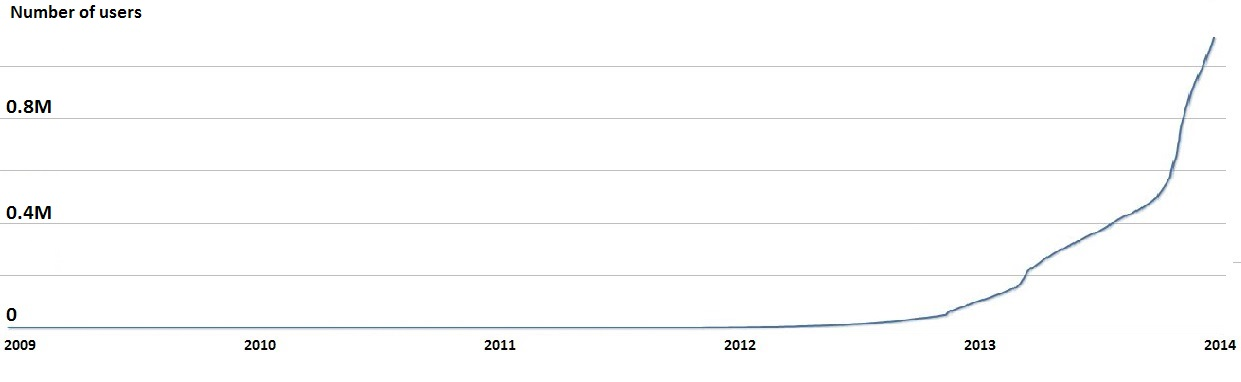
\includegraphics[width=10cm]{felhasznalok.jpg}
\caption{The number of users using online wallet.}
\end{center}
\end{figure}
\vspace{-0.5cm}

Assuming that the online wallet users already have to trust the web server, they more likely to trust a network of cooperating wallets such as the proposed lightweight bitcoin clients. According to our calculations above and the Figure 3., with only 1\% of the web client users use this new version will be feasible in the sense that their need to store sufficiently small amount of data. 

\subsection{Further problems}
The calculated results are not accurate since every transaction are stored at least in two places: the sender and the receiver (if none of them are the one who supposed to store the transaction, there are an additional player). So the 1.3 MB should be multiples by a factor less than 3, but this is still manageable amount. 

\newpage

It also really obvious that 3 client for all transaction would be not enough, it should be proportional to the number of transactions divided by the number of users. Further work is required on this topic including statistical data about the time a phone is connected in order to stochastically proximate the ration. 

An other issue is the distribution of the IDs. We use the IMEI numbers, which are unique for phones, but no other smart devices have them, This can solved by replacing it in these case with other unique identifier. 

% avoid double spending, attacks, level of trust in other nodes

\begin{thebibliography}{99}
\bibitem{}
https://en.bitcoin.it/wiki/Main\_Page
\label{bitcoinwiki}

\bibitem{}
http://en.wikipedia.org/wiki/Distributed\_hash\_table
\label{dhtwiki}

\bibitem{}
https://code.google.com/p/bitcoinj/
\label{bitcoinj}

\bibitem{}
http://bitcoin.org/bitcoin.pdf
\label{shatoshi}

\end{thebibliography}

\end{document}